\documentclass{bmd2016p}
\usepackage{epstopdf}

\newcommand{\e}{\ensuremath{\hat{\bm{e}}_1}}
\newcommand{\ee}{\ensuremath{\hat{\bm{e}}_2}}
\newcommand{\eee}{\ensuremath{\hat{\bm{e}}_3}}

\newcommand{\n}{\ensuremath{\hat{\bm{n}}_1}}
\newcommand{\nn}{\ensuremath{\hat{\bm{n}}_2}}
\newcommand{\nnn}{\ensuremath{\hat{\bm{n}}_3}}

\begin{document}

\begin{center}
\fontsize{14}{20}{\bf Buckling of the bicycle wheel}
\end{center}

%%%%%%%%%%%%%%%% authors %%%%%%%%%%%%%%%
\begin{center}
\normalsize{\bf{Matthew Ford$^{*}$, Jim M. Papadopoulos$^\#$, 
            Oluwaseyi Balogun$^\dag$}}
\end{center} 

\begin{center}
\begin{tabular}{c}
$^*$ Department of Mechanical Engineering\\
Northwestern University\\
2145 Sheridan Road, Evanston, IL 60208, USA\\
e-mail: mford@u.northwestern.edu\\[2.5ex]

$^\#$ Department of Mechanical and Industrial Engineering\\
Northeastern University\\
360 Huntington Ave., Boston, MA 02115, USA\\
e-mail: j.papadopoulos@northeastern.edu\\[2.5ex]

$^\dag$ Department of Civil Engineering\\
Northwestern University\\
2145 Sheridan Road, Evanston, IL 60208, USA\\
e-mail: o-balogun@northwestern.edu\\
\end{tabular}
\end{center}

\section*{ABSTRACT}
The spokes of a bicycle wheel brace and stiffen its slender rim, but only as long as the pre-tension is high enough to prevent them from going slack under external loads. However, above a certain critical spoke tension, the rim will buckle into a non-planar shape. Despite its importance for wheel strength and safety, there is no formula in the literature for the maximum tension a wheel can withstand before buckling.

Here we derive such a formula. The non-dimensionalized buckling tension depends only on two parameters which are identified as the ratio of rim torsional stiffness to rim bending stiffness, and the ratio of lateral spoke bracing stiffness to rim bending stiffness. The buckled rim adopts a sinusoidal lateral profile where the number of positive peaks $n\geq 2$ is determined by these two stiffness ratios. We show that the wheel may be represented by a system of equivalent springs: two series-connected springs for the rim bending and torsion stiffness, connected in parallel with a spring for the spoke system.

\begin{keywords}
bicycle wheel, 
bicycle safety, 
wheel strength, 
buckling, 
flexural-torsional.
\end{keywords}



\section{INTRODUCTION}
The earliest bicycles were built in the workshops of carriage makers who adapted the wheel technology of the time. These wheels typically had iron tires, wooden rims, and stout wooden spokes which bore the weight of the machine and rider in compression~\cite{Herlihy2004}. The spokes needed to be wide enough to prevent lateral buckling and to keep the rim planar, which made them very heavy and limited their maximum diameter. Around 1869, the tension-spoke wheel, an idea proposed in 1808 by Sir George Cayley but never realized, found its first application on the rapidly-developing bicycle~\cite{Ackroyd2011a,Clayton1991b}. Tangential-spoking was developed soon thereafter, and the typical bicycle wheel has not changed dramatically in form since then.

The tension-spoke wheel is a prestressed structure and is susceptible to buckling under internal forces. As the spokes are tightened uniformly, the rim shrinks radially under compression. At a critical spoke tension, the rim becomes unstable and buckles into a non-planar shape. The average spoke tension remains roughly constant after buckling and the original shape of the wheel can often be recovered by loosening the spokes. Buckling can also be triggered by external forces in an otherwise stable wheel leading to a release of strain energy. This process can lead to plastic yielding of the rim which makes wheel repair significantly more difficult.

Despite its implications for wheel strength, the buckling problem has never received a rigorous treatment to our knowledge. Jobst Brandt alludes to buckling due to uniform tension in his practical manual for wheelbuilders~\cite{Brandt1993c}:

\begin{quotation}
\noindent``If the wheel becomes untrue in two large waves during stress relieving, the maximum, safe tension has been exceeded. Approach this tension carefully to avoid major rim distortions. When the wheel loses alignment from stress relieving, loosen all spokes a half turn before retruing the wheel.''
\end{quotation}

He did not discuss the problem of buckling under tension further, but proposed that wheel failure commonly occurs due to lateral buckling when external loads have caused spokes to lose tension. Pippard and Francis~\cite{Pippard1932d} derived an equation for lateral deflection based on an elastic foundation model, but did not discuss stability and neglected the effect of spoke tension.

The theory of bicycle wheel buckling is closely related to the theory of flexural-torsional buckling of arches. Timoshenko and Gere~\cite{Timoshenko1961a} gave a formula for the critical load for a ring with doubly-symmetric cross-section subjected to radial loads. The theory of flexural-torsional buckling of monosymmetric arches (bicycle rim cross-sections generally have only one plane of symmetry) was broadly formalized by Trahair and Papangelis~\cite{Trahair1987b} using the virtual work approach to derive the equilibrium and stability equations. Their theory has been extended to treat arches restrained by continuous~\cite{Pi2002b} or discrete~\cite{Bradford2002d} elastic supports and elastic end restraints~\cite{Guo2014b}.

The problem of the prestressed bicycle wheel is unique for a number of reasons. First, buckling is caused by internal rather than external forces. Second, the spokes act both as elastic restraints resisting buckling and as prestressing elements causing buckling. Third, the lateral, radial, and torsional restraining actions of the spokes are coupled---i.e. lateral deflection of the rim may produce lateral, radial, and torsional reactions from the spokes. These considerations extend to other structural systems. Large observation wheels such as the London Eye~\cite{Mann2001a} and the Singapore Flyer~\cite{Allsop2009a} resemble large bicycle wheels with lateral stability due to the bracing angle of prestressed cables, and must be designed against flexural-torsional buckling.



\section{DEFORMATION OF THE WHEEL}
A typical bicycle wheel (Fig. \ref{fig:schematic}) consists of a slender rim connected to a hub by means of a system of very slender metal spokes. The spokes are usually threaded at the rim side into spoke nipples which are inserted through the rim from the outside. The spokes are kept under tension by the rim. Without pretension, the spokes would immediately buckle under a very small axial load due to their high aspect ratio.

\begin{figure}[!h]
\centering
\includegraphics[scale=1.0]{figures/bmd_figures-05.eps}
\caption{\textbf{(a)}-\textbf{(b)} Schematic of a model bicycle wheel. In general, the spokes lie on a hyperboloid which forms an angle of $\alpha$ with the wheel plane. If the in-plane angle $\beta$ is zero, the spoke surface is precisely a cone. \textbf{(c)} A wheel buckled into a saddle shape.}
\label{fig:schematic}
\end{figure}

To hold the spokes in tension, the rim must be under compression. An accurate approximation\footnote{95\% accurate for 6 spokes, $\alpha=10^{\circ}$, $\beta=10^{\circ}$, where angles $\alpha$ and $\beta$ are defined in Fig. \ref{fig:schematic}. Increasing the number of spokes only improves the estimate.} was given by Sharp~\cite{Sharp1977a} by considering a force balance on the top (or bottom) half of the rim.
	\begin{equation}\label{eq:TN}
	N_r = \frac{n_sT}{2\pi}
	\end{equation}
The spokes act like guy-wires, both supporting the rim radially and stabilizing the rim laterally. However, if the spoke tension exceeds a critical value $T_c$, the compression in the rim causes the wheel to buckle laterally, bending and twisting out of its initial plane, as shown in Fig. \ref{fig:schematic} (c).


\subsection{Rim equations}

The rim is modeled as an initially circular beam with a constant cross-section. For simplicity in this abbreviated treatment, we will assume that the shear center and centroid of the cross-section coincide. Except for warping deformation, plane cross-sections remain planar and transverse shear flexibility is neglected. Furthermore, we assume that the rim radius is much larger than the cross-sectional dimensions.

\begin{figure}[!ht]
\centering
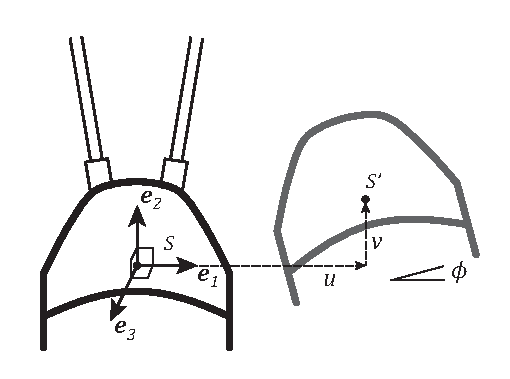
\includegraphics[scale=1.0]{figures/bmd_figures-06.eps}
\caption{Rim cross-section in the undeformed and deformed configuration. The shear center $S\rightarrow S'$ translates by the vector $\bm{u} = u\e + v\ee + w\eee$ and rotates through an angle $\phi$.}
\label{fig:def}
\end{figure}

The deformed configuration of the rim is described by the displacement of the shear center $\bm{u}=u\e + v\ee + w\eee$ and the twist angle $\phi$. The in-plane curvature $\kappa_1$ remains constant during flexural-torsional buckling. The in-plane curvature, out-of-plane curvature and twist rate are
	\begin{equation}\label{eq:k1}
	\kappa_1 = 1/R
	\end{equation}
	\begin{equation}\label{eq:k2}
	\kappa_2 = u'' - \frac{\phi}{R}
	\end{equation}
	\begin{equation}\label{eq:k3}
	\kappa_3 = \phi' + \frac{1}{R} u'
	\end{equation}
The symbol $()'$ indicates a derivative with respect to arc-length $s$ along the \eee{} direction. It can easily be verified that Equations \ref{eq:k1}--\ref{eq:k3} simplify to the standard equations for straight beams in the limit $R\rightarrow \infty$. The total strain energy is decomposed into lateral bending, uniform torsion, and warping terms which are related to the curvatures.
% The curvature and twist rate produce a bending moment and twisting moment equal to
	% \begin{equation}\label{eq:M2}
	% M_2 = EI_{11} \kappa_2
	% \end{equation}
	% \begin{equation}\label{eq:M3}
	% M_3 = GJ \kappa_3 + EI_w \kappa_3''
	% \end{equation}
	\begin{equation}\label{eq:Urim}
	U_{rim} = \frac{1}{2} \int_0^{2\pi} \left( EI_{11} \kappa_2^2 + GJ \kappa_3^2 + EI_w (\kappa_3')^2 \right)\, ds
	\end{equation}
The warping energy is primarily related to the bending energy in the rim sidewalls (which act as I-beam flanges) of the rim due to twisting\footnote{See http://www.steel-insdag.org/TeachingMaterial/Chapter17.pdf for a simple treatment.}. For a single-wall rim, the energy contribution from warping can exceed the contribution from torsion.

The length of a line segment of the rim is assumed to remain constant during buckling. The apparent shortening of an initial line segment $ds$ is given by the difference between $ds$ and $ds'$, the in-plane component of the deformed line segment.
	\begin{equation}\label{eq:ds}
	ds - ds' = ds - \sqrt{ds^2 - \left(\frac{du}{ds}ds\right)^2} \approx \frac{1}{2} (u')^2 \, ds
	\end{equation}
The axial compressive force in the rim moves through this displacement, performing virtual work equal to
	\begin{equation}\label{eq:Vrim}
	V_{rim} = \frac{1}{2} \int_0^{2\pi} N_r (u')^2 \, ds
	\end{equation}


\subsection{Spoke equations}

In this paper we consider bicycle wheels with slender prestressed spokes. We model a single spoke as an elastic bar pinned at each end, ensuring that the spoke force is always collinear with the spoke axis. The hub is assumed to be rigid. The linearized elongation of a spoke is given by
	\begin{equation}\label{eq:selong}
	\Delta l = \bm{u}_n\cdot \n
	\end{equation}
where $\bm{u}_n$ is the displacement vector of the spoke nipple and \n{} is a unit vector pointing along the axis of the spoke. The linearized rotation of the spoke is given by
	\begin{equation}\label{eq:srot1}
	\Omega_1 = \frac{1}{l} \bm{u}_n\cdot \nn
	\end{equation}
	\begin{equation}\label{eq:srot2}
	\Omega_2 = \frac{1}{l} \bm{u}_n\cdot \nnn
	\end{equation}
where \nn{} and \nnn{} are two orthogonal unit vectors orthogonal to \n{}, and $l$ is the spoke length. The elongation produces a net force on the rim parallel to the original spoke axis equal to
	\begin{equation}\label{eq:sF1}
	f_1 = E_sA_s\left(\frac{\Delta l}{l}\right)\n = \frac{E_sA_s}{l} \n \cdot \bm{u}_n 
	\end{equation}
The rotation of the spoke produces net forces on the rim perpendicular to the original spoke axis due to the rotation of the initial tension vector.
	\begin{equation}\label{eq:sF2}
	f_2 = T \sin{\Omega_1} \approx \frac{T}{l} \nn \cdot \bm{u}_n
	\end{equation}
	\begin{equation}\label{eq:sF3}
	f_3 = T \sin{\Omega_2} \approx \frac{T}{l} \nnn \cdot \bm{u}_n
	\end{equation}
since \n{}, \nn{}, \nnn{} are mutually orthogonal, the total force on the rim is given by $\bm{f} = \bm{k}_f \cdot \bm{u}_n$, where the spoke stiffness matrix is given by
	\begin{equation}\label{eq:kf}
	\bm{k}_f = \frac{E_sA_s}{l}\n\n + \frac{T}{l}(\nn\nn + \nnn\nnn)
	\end{equation}
The first term in Eqn.~\ref{eq:kf} is the {\bf elastic stiffness} and the second term is the {\bf tension stiffness}. The tension stiffness is the component responsible for the transverse vibrations of a guitar string, e.g. The term $\n\n$ is the dyadic product, or tensor product (also called the outer product), and is defined by the property $\n\n\cdot \bm{a} = (\n\cdot \bm{a})\n$ for any vector $\bm{a}$.

Formalizing the approach of Smith~\cite{Smith1901a} and Pippard~\cite{Pippard1932d}, we will approximate the spoke system as a continuous elastic ``disc'' which exerts a distributed load on the rim. The stiffness per unit length is given by the sum of the spoke stiffnesses in one periodic grouping of $n_p$ spokes, divided by the arc length of the grouping\footnote{For a conventional cross-laced wheel, $n_p=4$: drive-side pulling spoke, drive-side trailing spoke, left-side pulling spoke, left-side trailing spoke. For a radial-spoked wheel, $n_p=2$: drive-side spoke, left-side spoke.}.
	\begin{equation}\label{eq:kbar}
	\bar{\bm{k}} = \frac{1}{2\pi R}\left(\frac{n_s}{n_p}\right) \sum_i^{n_p} \bm{k}_{f, i}
	\end{equation}
	The distributed load $\bar{\bm{f}}$ does an amount of work per unit length equal to
	\begin{equation}\label{eq:w_spokes}
	\bar{w} = \int_0^{\bm{u}_n} \bar{\bm{f}} \cdot d\bm{u}_n = \frac{1}{2} \bm{u}_n \cdot \bar{\bm{k}} \cdot \bm{u}_n
	\end{equation}
Each spoke is assumed to terminate at the rim shear center. Therefore $\bm{u}_n = \bm{u}$. Substituting a lateral buckling displacement $\bm{u}=u\e$ into Eqn. \ref{eq:w_spokes} and integrating over the length of the rim gives the strain energy stored in the spoke system.
	\begin{equation}\label{eq:Us}
	U_{spokes} = \int_0^{2\pi} \bar{w} \, ds = \frac{1}{2} \bar{k}_{uu}u^2
	\end{equation}
The continuum spoke stiffness can be written $\bar{\bm{k}} = \bar{\bm{k}}^{el} + \bar{\bm{k}}^{tens}$, where the second term is proportional to $T$. A very close approximation for the lateral component $\bar{k}_{uu}$ for a symmetrically dished wheel is given by
	\begin{equation}\label{eq:kuu}
	\bar{k}_{uu} = \frac{n_sE_sA_s}{2\pi Rl}\sin^2{\alpha} + \frac{n_s T}{2\pi Rl}
	\end{equation}


\subsection{Total potential energy and buckling criterion}
The wheel becomes unstable when the increase in strain energy is exactly balanced by the virtual work for a perturbing displacement $\delta u, \delta\phi$, i.e. when the total potential energy is zero.
	\begin{equation}\label{eq:TotPot}
	\Pi = U_{rim} + U_{spokes} - V_{rim} = 0
	\end{equation}
We assume a buckled shape of the form
	\begin{equation}\label{eq:modeshape}
	\begin{split}
	u &= \delta u_n \cos{\frac{ns}{R}} \\
	\phi &= \delta\phi_n \cos{\frac{ns}{R}}
	\end{split}
	\end{equation}
\,\,\,\, where $n$ is the number of positive peaks of the lateral displacement. Substituting the buckling mode shape Eqn. \ref{eq:modeshape} into Eqns. \ref{eq:Urim}, \ref{eq:Vrim}, and \ref{eq:Us} and substituting into Eqn. \ref{eq:TotPot} yields a buckling criterion for the $n$th mode.
	\begin{multline}\label{eq:ECrit}
	\frac{\pi EI_{11}}{R^3}(n^2 \delta u_n - R\delta\phi_n)^2 + \frac{\pi n^2}{R^2}\left(GJ + \frac{EI_w}{R^2}n^2\right)(\delta u_n-R\delta\phi_n)^2 + \\
	\pi R(\bar{k}_{uu}^{el} + \bar{k}_{uu}^{el})\delta u_n^2 - N_r\frac{\pi n^2}{R}\delta u_n^2=0
	\end{multline}
The torsional stiffness and warping stiffness can be combined into an effective torsional stiffness $\widetilde{GJ} = GJ + n^2EI_w/R^2$. Equation \ref{eq:ECrit} has a quadratic form and can be written in matrix notation:
	\begin{equation}\label{eq:Qform}
	\begin{bmatrix}
	\delta u_n\\\delta\phi_n
	\end{bmatrix} \cdot
	\begin{bmatrix}
	\frac{\partial^2 \Pi}{\partial u_n^2} & \frac{\partial^2 \Pi}{\partial u_n \partial \phi_n}\\
	\frac{\partial^2 \Pi}{\partial u_n\partial\phi_n} & \frac{\partial^2 \Pi}{\partial \phi_n^2}
	\end{bmatrix} \cdot
	\begin{bmatrix}
	\delta u_n\\\delta\phi_n
	\end{bmatrix}
	=0
	\end{equation}
Non-trivial solutions of Eqn. \ref{eq:Qform} exist when the determinant of the matrix vanishes. Expanding the determinant in Eqn. \ref{eq:Qform} and substituting Eqns. \ref{eq:TN} and \ref{eq:kuu} yields a linear equation for the critical buckling tension of the $n$th mode.
	\begin{multline}\label{eq:Tc_eq}
	\left(\frac{2\pi EI_{11}}{R}+\frac{2\pi \widetilde{GJ}n^2}{R} \right) \left( \frac{2\pi \widetilde{GJ}n^2}{R^3} + \frac{2\pi EI_{11}n^4}{R^3} + 2\pi R\bar{k}_{uu}^{el} + \frac{n_sT_{cn}}{l} - \frac{n_sn^2T_{cn}}{R}\right)\\
	- \left( \frac{2\pi EI_{11}n^2}{R^2} + \frac{2\pi \widetilde{GJ}n^2}{R^2} \right)^2 = 0
	\end{multline}
Solving Eqn. \ref{eq:Tc_eq} for $T_{cn}$ yields the tension at which the $n$th mode becomes unstable. The critical buckling tension $T_c$ is the minimum $T_{cn}$ with respect to the mode number $n\geq 2$.



\section{BUCKLING DUE TO SPOKE TENSION}
The solution to Eqn. \ref{eq:Tc_eq} can be written in non-dimensional form as
	\begin{equation}\label{eq:Tc_nondim}
	\frac{T_{cn}}{T_e} = \left( \frac{\tilde{u}n^2(n^2-1)^2}{1+\tilde{\mu}n^2} + \lambda \right) \left(\frac{1}{n^2-R/l} \right)
	\end{equation}
\,\,\,\, where the ``Euler tension'' $T_e=2\pi EI_{11}/n_sR^2$ is the tension that would produce a compressive force in the rim equal to the classical buckling load for a straight beam-column of length $2\pi R$. The parameter $\tilde{\mu} = \widetilde{GJ}/EI_{11}$ is the ratio of the effective torsional stiffness to the lateral bending stiffness. The parameter $\lambda = \bar{k}_{uu}^{el}R^4/EI_{11}$ is the ratio of the spoke system stiffness $\bar{k}_{uu}^{el}R$ to the rim bending stiffness $EI_{11}/R^3$. For most wheels, $R/l\approx 1$.

\begin{figure}[!ht]
\centering
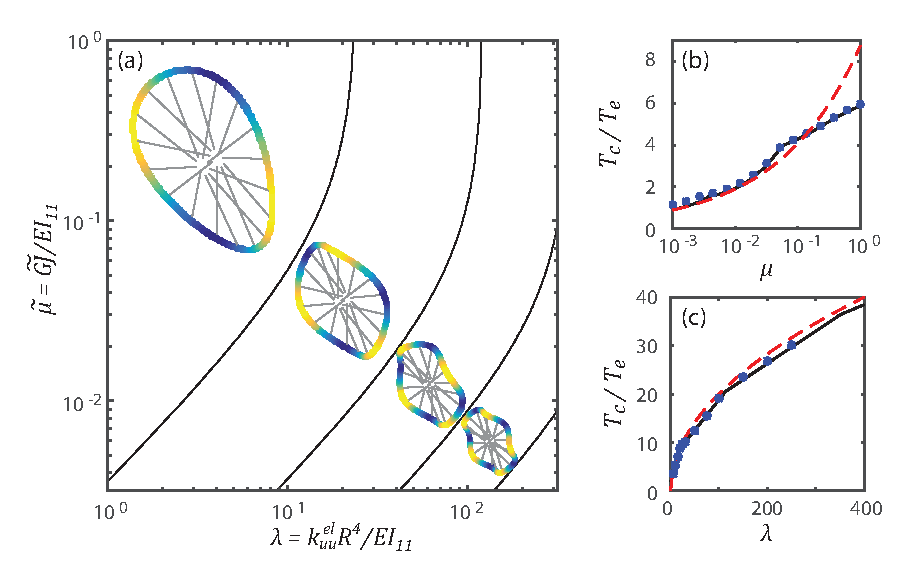
\includegraphics[scale=1.0]{figures/bmd_figures-04.eps}
\caption{\textbf{(a)} Buckling mode parameter map showing the lowest-energy buckling mode in each region. \textbf{(b)}--\textbf{(c)} Normalized buckling tension vs. $\tilde{\mu}$ and $\lambda$. Solid black line: Eqn. \ref{eq:Tc_nondim}, dashed red line: power law, blue stars = finite-element calculations. (a) $\lambda=10$, (b) $\tilde{\mu} = 0.38$.}
\label{fig:Tc_nondim}
\end{figure}

Since $n$ is a discrete variable, there is no closed-form expression for the minimum $T_{cn}$ for a given $(\tilde{\mu},\lambda)$. The minimum-energy buckling mode must be found by comparing $T_{cn}$ for the first several modes and taking the smallest value (see Fig. \ref{fig:Tc_nondim} (a)). However, two important \textit{approximate} solutions can be derived by replacing the discrete mode number $n$ with a continuous variable $\bar{n}$ and minimizing Eqn. \ref{eq:Tc_nondim} analytically, resulting in two simple power laws for $T_c$.


\subsection{Rims with low torsional stiffness}\label{sec:powerlaw_1}
Many bicycle rims are built from thin-walled open channel sections which have very low torsional stiffness $\widetilde{GJ}$ compared with their bending stiffness. Replacing the discrete mode number $n$ with a continuous variable $\bar{n}$, we adopt the following ansatz: (a) $\bar{n}^2 \gg 1$ and (b) $\tilde{\mu}\bar{n}^2 \ll 1$. Under these conditions, Eqn. \ref{eq:Tc_nondim} becomes
	\begin{equation}\label{eq:Tcn_small_mu}
	T_{cn} = \frac{2\pi EI_{11}}{n_sR^2} \left( \tilde{\mu}\bar{n}^4 + \frac{\lambda}{\bar{n}^2}\right)
	\end{equation}
Minimizing Eqn. \ref{eq:Tcn_small_mu} with respect to $\bar{n}$ by setting the derivative $dT_{cn}/d\bar{n}=0$, we obtain the scaling law
	\begin{equation}\label{eq:nbar_small_mu}
	\bar{n} = \left(\frac{\lambda}{2\tilde{\mu}} \right)^{1/6}
	\end{equation}
Substituting Eqn. \ref{eq:nbar_small_mu} into Eqn. \ref{eq:Tcn_small_mu} yields a power law for $T_c$.
	\begin{equation}\label{eq:Tc_small_mu}
	T_c \approx \frac{11.875}{n_sR^2} \, \left(\bar{k}_{uu}^{el}R^4 \right)^{2/3} (\widetilde{GJ})^{1/3}
	\end{equation}
Equation \ref{eq:Tc_small_mu} suggests that when the torsional stiffness is smaller than the bending stiffness, the buckling behavior is dominated by torsion and does not depend explicitly on the bending stiffness at all. Equation \ref{eq:Tc_small_mu} is shown in Fig. \ref{fig:Tc_nondim} next to Eqn. \ref{eq:Tc_nondim} and finite-element calculations. The power law is strictly less than Eqn. \ref{eq:Tc_nondim} which conveniently gives a conservative design criterion.


\subsection{Lateral stiffness of spoke system much greater than rim bending stiffness}
A second power law regime appears when $\lambda \gg 1$ and $\tilde{\mu} \sim 1$. Under these conditions, Eqn. \ref{eq:Tc_nondim} becomes
	\begin{equation}\label{eq:Tcn_boef}
	T_{cn} = \frac{2\pi EI_{11}}{n_sR^2}\left(\bar{n}^2 + \frac{\lambda}{\bar{n}^2} \right)
	\end{equation}
Following the same procedure in section \ref{sec:powerlaw_1} gives another separate power law:
	\begin{equation}\label{eq:Tc_boef}
	T_c \approx \frac{4\pi}{n_s} \left(\bar{k}_{uu}^{el}EI_{11} \right)^{1/2} 
	\end{equation}
Substituting Eqn. \ref{eq:TN} for $T_c$ gives $N_{rc}=2\left(\bar{k}_{uu}^{el}EI_{11}\right)^{1/2}$, which is precisely the buckling load for an infinite, straight beam on an elastic foundation~\cite{Hetenyi1946b}. Figure \ref{fig:Tc_nondim} (c) shows a comparison of Eqn. \ref{eq:Tc_boef} against Eqn. \ref{eq:Tc_nondim} and finite-element calculations.



\section{EQUIVALENT SPRING MODEL}
The form of Eqn. \ref{eq:Tc_nondim} suggests that the buckling tension is governed by an equivalent stiffness which combines the bending stiffness and torsion stiffness of the rim and the lateral stiffness of the spoke system. Here we will describe an equivalent system of linear springs (Fig. \ref{fig:Kn}) consisting of two springs connected in series representing the torsion and bending stiffnesses of the rim, in parallel with a single spring representing the lateral stiffness of the spoke system.

The lateral stiffness of the wheel can be decomposed into orthogonal modes in the form of Eqn. \ref{eq:modeshape}. Since the Fourier modes are orthogonal, the total strain energy is the sum of the strain energies in each mode.
	\begin{equation}\label{eq:Umode}
	U_{total} = U_0 + U_1 + U_2 + ...
	\end{equation}

\begin{figure}[!ht]
\centering
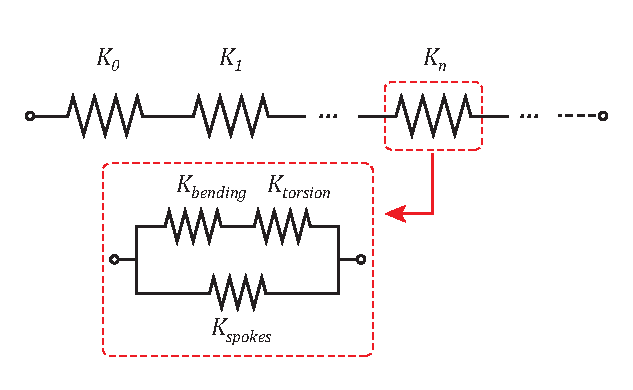
\includegraphics[scale=1.0]{figures/bmd_figures-03.eps}
\caption{Equivalent spring model. Each mode stiffness consists of three equivalent springs representing the rim bending and torsion stiffness and the spoke stiffness.}
\label{fig:Kn}
\end{figure}

The applied lateral force and torque are determined using Castigliano's first theorem. For an applied force $P$ and no applied torque, we have
	\begin{equation}\label{eq:Castig}
	\begin{split}
	P &= \frac{\partial U_n}{\partial u_n}\\% = \frac{\partial^2 U_n}{\partial u_n^2}u_n + \frac{\partial^2 U_n}{\partial u_n \partial \phi_n}\phi_n\\
	0 &= \frac{\partial U_n}{\partial \phi_n}% = \frac{\partial^2 U_n}{\partial \phi_n^2}\phi_n + \frac{\partial^2 U_n}{\partial \phi_n \partial u_n}u_n
	\end{split}
	\end{equation}
Substituting $U_{rim} + U_{spokes}$ for $U_n$ and inserting the mode shape Eqn. \ref{eq:modeshape}, Eqn. \ref{eq:Castig} becomes a linear system of equations for $u_n$ and $\phi_n$. Solving \ref{eq:Castig} for $u_n$ yields
	\begin{equation}\label{eq:un}
	u_n = \left(\frac{PR^3}{\pi}\right) \frac{EI_{11}+\widetilde{GJ}n^2}{EI_{11}\widetilde{GJ}n^2(n^2-1)^2 + R\bar{k}_{uu}(EI_{11}+\widetilde{GJ}n^2)}
	\end{equation}
Defining an equivalent torsion stiffness, bending stiffness, and spoke stiffness, the mode stiffness $P/u_n$ can be obtained from Eqn. \ref{eq:un} as
	\begin{equation}\label{eq:Kn_spring}
	K_n = \frac{K_{bending}K_{torsion}}{K_{bending}+K_{torsion}} + K_{spokes}
	\end{equation}
\,\,\,\, where
	\begin{equation}\label{eq:Ktorsion}
	K_{torsion} = \frac{\pi\widetilde{GJ}n^2}{R^3}(n^2-1)^2
	\end{equation}
	\begin{equation}\label{eq:Kbending}
	K_{bending} = \frac{\pi EI_{11}}{R^3}(n^2-1)^2
	\end{equation}
	\begin{equation}\label{eq:Kspokes}
	K_{spokes} = \pi R \bar{k}_{uu}^{el}
	\end{equation}
The form of Equation \ref{eq:Kn_spring} suggests an equivalent spring model (Fig. \ref{fig:Kn}) for the $n$th mode in which the rim stiffness is represented by two springs connected which is then connected in parallel with the spoke stiffness. If there is a large difference between the rim bending stiffness and torsion stiffness, the equivalent rim stiffness will be dominated by the smaller of the two.

With this definition, the critical buckling tension for the $n$th mode (Eqn. \ref{eq:Tc_nondim}) has an extremely simple form
	\begin{equation}\label{eq:Tc_Kn}
	T_{cn} = \frac{2RK_n}{n_s(n^2 - R/l)}
	\end{equation}
In this form, the benefit of adding spoke stiffness becomes readily apparent. Because the rim stiffness and spoke stiffness act in parallel, increasing either one directly impacts the maximum tension.



\section{FINITE-ELEMENT CALCULATIONS}
We validated our theoretical predictions against non-linear finite-element calculations implemented in ABAQUS\textsuperscript{\textregistered} 6.14\footnote{ABAQUS\textsuperscript{\textregistered} is a registered trademark of Dassault Syst\`emes.}. The spokes and rim were both modeled using 2-node linear beam elements including shear flexibility (element type B31 in the ABAQUS library). The rim was interpolated with sufficient elements such that any given beam segment spanned less than 6$^{\circ}$ of the circle (e.g. 2 rim elements between each spoke for a 36-spoke wheel). Each spoke was modeled with 10 beam elements to accurately reproduce local spoke buckling.

A controlled tensioning strain was applied to the spokes by defining a coefficient of thermal expansion of 1.0 for the spokes (but not the rim) and ramping the temperature down to 150\% of the expected critical buckling strain. The initial rim shape was given a geometric imperfection by perturbing the lateral coordinate of the rim nodes by $\cos{ns/R}$. Imperfections starting with $n=2$ up to the expected buckling mode were included. The solution was obtained via an implicit integration procedure (ABAQUS Standard) including non-linear geometric effects.

\begin{figure}[!ht]
\centering
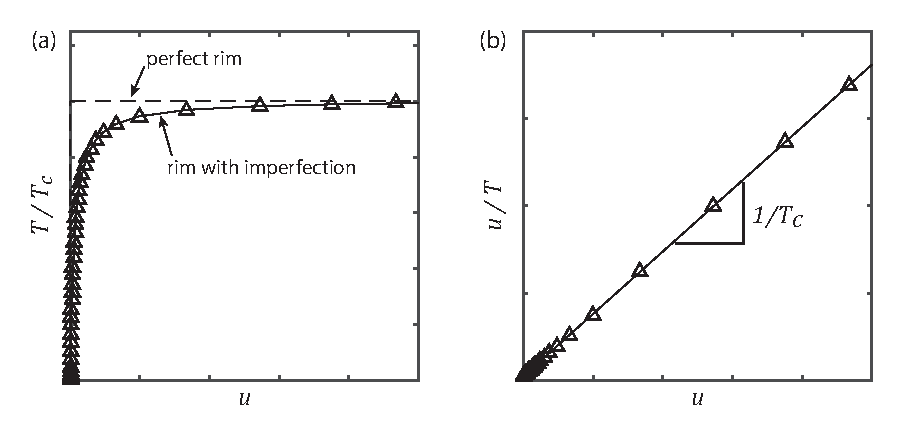
\includegraphics[scale=1.0]{figures/bmd_figures-07.eps}
\caption{\textbf{(a)} Normalized spoke tension vs. lateral deflection. \textbf{(b)} Southwell plot for a simulated wheel with an imperfection.}
\label{fig:Southwell}
\end{figure}

The average spoke tension was recorded at each loading step. The buckling tension was determined from a Southwell plot~\cite{Timoshenko1961a} of $u/T$ vs. $u$, where $u$ is taken at its maximum location on the rim. The deflection of a loaded structure with an initial imperfection is approximately
	\begin{equation}\label{eq:Southwell}
	u = \frac{a}{T_c/T - 1}
	\end{equation}
Therefore the slope of $u/T$ vs. $u$ is $1/T_c$. The buckling tension was also calculated by finding the strain at which the average tension departs from linearity by more than 3\%. The two methods were found to give results in very close agreement.



\section{CONCLUSIONS}
The bicycle wheel relies on spoke tension to support external loads. As a rule-of-thumb, a typical wheel can withstand a radial load of approximately $2T$ before the bottom-most spokes lose tension. Therefore, higher tension is desirable to increase the strength of the wheel. However, we have shown that if the spoke tension is too high, the rim becomes unstable under internal forces, without even considering external loads. Tension---the property which gives a wheel its strength---can also be its downfall.

Our theory points towards some practical design rules: \textbf{(1)} Since the rim bending stiffness and torsional stiffness effectively act like springs in series, the more flexible mode will dominate. Therefore they should be in relative balance. Modern double-walled rims are advantageous in this respect because of their closed cross-section, while classic single-walled rims are much more flexible in torsion than in bending. \textbf{(2)} Since the rim and spoke stiffnesses act like springs in parallel, they can both be increased to roughly equal effect. \textbf{(3)} Since the lateral spoke stiffness scales as $\sin^2{\alpha}$, the most significant factor affecting the spoke stiffness is the cone angle $\alpha$. Even a modest increase in hub width can increase the stiffness and buckling tension dramatically, while having negligible effect on the radial stiffness.

The spokes give a significant contribution to the buckling resistance of bicycle wheels. The spoke system lateral stiffness (Eqn. \ref{eq:kuu}) scales directly with the elastic modulus (material-dependent, but not alloy-dependent) and the cross-sectional area, and inversely with the spoke length (which varies only slightly depending on spoke pattern). It is counter-intuitive that increasing the number of spokes actually slightly \textit{decreases} the buckling tension (due to the factor of $n_s$ appearing in $T_e$ in Eqn. \ref{eq:Tc_nondim}). However, increasing the number of spokes also reduces the fraction of load transferred to a single spoke and thus reduces the required tension. The net effect is that more spokes results in a stronger wheel.

One might wonder, why do practically all wheels fail in the $n=2$ mode, when higher modes are possible? We offer three speculative possibilities: \textbf{(1)} the geometry and stiffness of wheels are such that most wheels fall into the $n=2$ regime of Fig. \ref{fig:Tc_nondim}. \textbf{(2)} Wheels which would buckle into higher modes typically fail in other manners first (such as spoke yielding or nipple fracture). \textbf{(3)} Rim failure is usually accompanied by spoke buckling, which reduces the effective wheel stiffness and in turn favors the $n=2$ mode. Preliminary non-linear finite-element simulations of wheel failure under external loads provide some evidence for (3), but more work is required to apply our analysis to real-world wheels.



\section*{ACKNOWLEDGEMENTS}
This material is based upon work supported by the National Science Foundation Graduate Research Fellowship Program under Grant No. DGE-1324585. Any opinions, findings, and conclusions or recommendations expressed in this material are those of the authors and do not necessarily reflect the views of the National Science Foundation.


\normalem
\bibliographystyle{naturemag}
\bibliography{C:/Users/matt/OneDrive/Documents/Research/bibtex/Papers-BMD2016.bib}


\newpage
\section*{LIST OF TERMS}

\begin{table}[ht!]
\caption{A partial list of symbols is given below. Other symbols are defined in-place or not re-used.}
\begin{tabular}{c|p{12cm}}
\hline
\textit{\textbf{Term}} & \textit{\textbf{Definition}} \\
\hline
$n_s$		& Number of spokes\\
$E_s, A_s$	& Spoke Young's modulus and cross-sectional area\\
$l$			& Spoke length\\
$\alpha$	& Out-of-plane spoke angle--wall angle of a hypothetical ``cone'' of spokes\\
$\beta$		& In-plane spoke angle--measured between the in-plane projection of the spoke and
			  a radius of the wheel\\
$\n$		& Unit vector aligned with the spoke axis\\
$\nn,\nnn$	& Two unit vectors perpendicular to the spoke axis\\
$\bm{f}$	& Force exerted by a spoke on the rim\\
$\bar{\bm{f}}$& Distributed force (per-unit-length) exerted by the spokes on the rim\\
$f_1, f_2,f_3$ & Vector components of $\bm{f}$\\
$\bm{k}_f$	& Stiffness matrix for a single spoke\\
$\bar{\bm{k}}$ & Equivalent stiffness per-unit-length of the spoke system. $\bar{\bm{k}} = \bar{\bm{k}}^{el} + \bar{\bm{k}}^{tens}$\\
$\bar{\bm{k}}^{el},\bar{\bm{k}}^{tens}$ & Part of $\bar{\bm{k}}$ proportional to $E_sA_s$ and $T$, respectively\\
$\bar{k}_{ij}$ & Matrix components of $\bar{\bm{k}}$\\
$\e,\ee,\eee$ & Coordinate axes defined at the rim shear center\\
$s$			& Arc-length coordinate along the rim\\
$\kappa_1,\kappa_2,\kappa_3$ & Spatial curvature of the rim\\
$\bm{u}$	& Displacement of the rim shear center\\
$u,v,w$		& Vector components of $\bm{u}$ in the \e{}, \ee{}, \eee{} directions.\\
$\phi$		& Rotation of the rim cross-section about the $\hat{\bm{e}}_3$ axis.\\
$\delta u, \delta \phi$ & Virtual displacement and rotation\\
$\delta u_n, \delta\phi_n$ & Buckling mode coefficients\\
$n$			& Buckling mode number\\
$U_{rim}$	& Strain energy in the rim due to buckling\\
$V_{rim}$	& Virtual work of internal forces in the rim\\
$U_{spokes}$& Strain energy in the spokes due to buckling\\
$T$			& Tension in a spoke\\
$T_{cn}$	& Critical spoke tension for the $n$th mode\\
$T_c$		& Critical buckling tension (minimum of $T_{cn}$ over all modes)\\
$T_e$		& ``Euler'' tension--tension which would produce an axial force in the rim
			  equal to the buckling load for a straight beam-column of length $2\pi R$\\
$R$			& Rim radius measured from the rim shear center\\
$E, G$		& Rim Young's modulus and shear modulus\\
$I_{11}$	& Second moment of area of the rim in the lateral direction\\
$J$			& Rim torsion constant\\
$I_w$		& Rim warping constant\\
$\widetilde{GJ}$ & Effective torsional rigidity including both Saint-Venant torsion and warping\\
$\tilde{\mu}$ & Ratio of effective torsional rigidity to bending rigidity: $\widetilde{GJ}/EI_{11}$\\
$\lambda$	& Ratio of spoke system lateral stiffness to rim bending stiffness OR ratio
			  of rim radius to the characteristic length of a beam on an elastic foundation.\\
\hline
\end{tabular}
\end{table}


\newpage
\section*{FINITE-ELEMENT RESULTS}
For all the following wheels: $R=0.3$ m, $EI_{11}=EI_{22}=69.0$ N-m$^2$, $GJ=26.0$ N-m$^2$, $I_w=0$, $E_s=210$ GPa. The cross-sectional area of the rim is 100 mm$^2$. All length measurements in the following table are given in mm. $T_c$ is reported in Newtons. Hub flange width is the distance from the drive-side flange to the left-side flange. Hub flange diameter is the diameter of the circle that passes through the centers of the spoke eyelets.

\begin{table}[ht!]
\caption{Parameters for FEA simulations shown in Fig \ref{fig:Tc_nondim} (b).}
\begin{tabular}{c|c|c|c|c|c}
\hline
$n_s$	& Spoke diameter	& Hub flange width	& Hub flange diameter	& $T_c$ ABAQUS	& $T_c$ theory\\
\hline
36		& 0.693				& 50				& 40					& 477			& 475\\
36		& 0.981				& 50				& 40					& 668			& 704\\
\hline
48		& 1.040				& 50				& 40					& 694			& 698\\
48		& 1.201				& 50				& 40					& 862			& 870\\
48		& 1.343				& 50				& 40					& 956			& 942\\
48		& 1.471				& 50				& 40					& 1021			& 1005\\
48		& 1.900				& 50				& 40					& 1270			& 1259\\
48		& 1.943				& 60				& 40					& 1563			& 1573\\
\hline
64		& 1.671				& 60				& 40					& 1450			& 1418\\
\end{tabular}
\end{table}

For all the following wheels: $n_s=36$, $R=0.3$ m, hub flange width = $50$ mm, hub flange diameter = $40$ mm, spoke diameter = $0.981$ mm, $EI_{11}=EI_{22}=69.0$ N-m$^2$, $I_w=0$, $E_s=210$ GPa. $GJ$ varies with $\mu$ given in the table below. The cross-sectional area of the rim is 100 mm$^2$. $T_c$ is reported in Newtons.

\begin{table}[ht!]
\centering
\caption{Parameters for FEA simulations shown in Fig \ref{fig:Tc_nondim} (c).}
\begin{tabular}{c|c|c}
\hline
$\mu$	& $T_c$ ABAQUS & $T_c$ theory\\
\hline
0.001	& 154	& 121 \\
0.00215	& 191	& 157 \\
0.00464	& 220	& 212 \\
0.01	& 264	& 258 \\
0.0215	& 359	& 344 \\
0.0464	& 501	& 487 \\
0.1		& 556	& 574 \\
0.215	& 624	& 646 \\
0.464	& 701	& 723 \\
1		& 759	& 785 \\
\end{tabular}
\end{table}

\end{document}
